\chapter{Wdrożenie systemu w chmurze obliczeniowej}

Wyróżnia się kilka podstawowych etapów niezbędnych do prawidłowego wdrożenia systemu:

\begin{enumerate}
    \item Przygotowanie dokumentacji.
    \item Ustawienie infrastruktury.
    \item Przygotowanie środowiska testowego.
    \item Testy systemu.
    \item Migracja danych.
    \item Uruchomienie systemu produkcyjnego.
\end{enumerate}

W mojej pracy skupiłem się na dwóch punktach: ustawienia infrastruktury oraz przygotowania środowiska testowego. Zostało to zrealizowane w chmurze ze względu na redukcję kosztów oraz skalowalność rozwiązania. Nie wymaga to od dostawcy oprogramowania własnej infrastruktury oraz pozwala na sprawne zarządzanie posiadanymi zasobami.

System kategoryzacji korzysta z trzech usług zlokalizowanych na platformie Amazon Web Services:

\begin{enumerate}
    \item API gateway
    
    Bramka, która zajmuje się przyjmowaniem żądań użytkownika i przekazywanie ich do odpowiedniego serwisu. API Gateway w systemie klasyfikacji przyjmuje żądanie HTTP od użytkownika i przekazuje je do funkcji działającej w usłudze AWS Lambda.
    
    \item AWS Lambda
    
    Usługa pozwalająca na uruchamianie własnego kodu użytkownika w postaci funkcji. Uruchamianie może być wywołane ręcznie lub poprzez inny serwis AWS. W systemie klasyfikacji uruchomienie funkcji wywoływane jest przez serwis API Gateway.
    
    \item DynamoDB
    
    Baza danych zorientowana dokumentowo przechowywująca dane w postaci klucz-wartość. Obszerwnie opisana w rozdziale \ref{cha:wprowadzenieTechnologiczne}.
\end{enumerate}

\newpage
\begin{figure}[H]
    \centering
    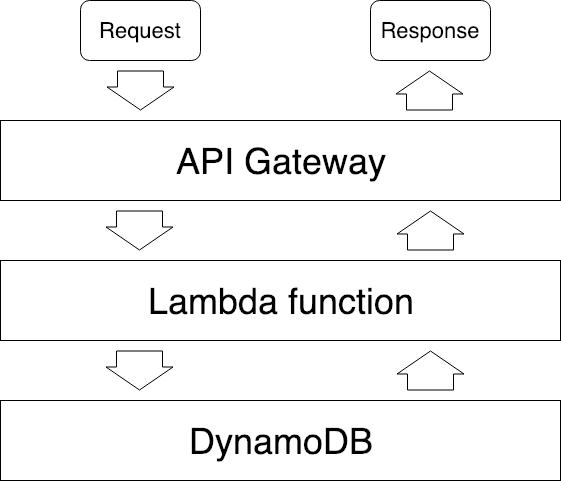
\includegraphics[width=10cm]{images/wdrozenie/aws_Architecture.png}
    \caption{Architektura infrastruktury systemu wdrożonego na platformie Amazon Web Services}
    \label{fig:architecture}
    \end{figure}

\section{AWS Lambda - wdrażanie aplikacji w środowisku serverless}

Lambda oferuje nam moc obliczeniową bez potrzeby dostarczania oraz zarządzania serwerami. Amazon dostarcza nam całe potrzebne środowisko - naszym zadaniem jest jedynie przekazanie kodu, który ma być uruchamiany. Za skalowanie oraz administrację środowiskiem odpowiedzialny jest dostawca usług.

Umieszczenie dużej aplikacji w usłudze AWS Lambda nie jest prostym wyzwaniem. Sporym ograniczeniem jest maksymalny rozmiar spakowanego kodu - 50MB. Serwis klasyfikacji z racji zależności z bibliotekami do obliczeń (numpy i scikit-learn) oraz zestawu słów do przetwarzania języka naturalnego osiąga ponad dwukrotnie większy rozmiar. 

Problemy z ograniczeniami usługi AWS Lambda rozwiązałem posługując się projektem Zappa \footnote{https://github.com/Miserlou/Zappa}. Pozwolił on na zautomatyzowanie następujących czynności:

\begin{enumerate}
    \item Spakowanie aplikacji wraz ze wszystkimi dependencjami kompatybilnymi ze środowiskiem AWS Lambda w plik zip.
    
    \item Utworzenie odpowiednich uprawnień do innych zasobów platformy AWS.
    
    \item Utworzenie funkcji AWS Lambda ze spakowanym kodem.
    
    \item Utworzenie API Gateway odpowiedzialnego za komunikację z funkcją AWS Lambda.
\end{enumerate}

Ograniczenie wielkości spakowanego kodu zostało ominięte dzięki opcji 'slim\_handler' \footnote{https://github.com/Miserlou/zappa-blog/blob/master/posts/slim-handler.md}. Gdy jej używamy - do funkcji AWS Lambda przekazywana jest jedynie minimalna ilość kodu, a reszta wysłana zostaje do serwisu AWS Simple Storage Service (S3) \footnote{https://aws.amazon.com/s3/}. Gdy następuje tzw. 'cold start', czyli pierwsze uruchomienie aplikacji na nowej maszynie - wtedy reszta kodu jest na nią pobierana do tymczasowej lokacji i wykonywana przy każdym odwołaniu z API Gateway. Wadą takiego rozwiązania jest wydłużony czas wykonywania pierwszego zapytania do API - wtedy właśnie reszta kodu musi zostać pobrana.

Dodatkowym aspektem wdrożenia projektu była integracja apikacji działającej w środowisku serverless z bazą danych. Aplikacja komunikuje się z bazą DynamoDB wykorzystując AWS SDK, jednak, aby korzystać z jej zasobów muszą zostać zdefiniowane odpowiednie uprawnienia. W konfiguracji projektu Zappa znalazły się one w sekcji 'extra\_permissions':

\begin{verbatim}
    "extra_permissions": [
      {
        "Effect": "Allow",
        "Action": [
          "dynamodb:DeleteItem",
          "dynamodb:GetItem",
          "dynamodb:PutItem",
          "dynamodb:UpdateItem",
          "dynamodb:Scan",
          "dynamodb:Query",
          "dynamodb:ListTables",
          "dynamodb:CreateTable",
          "dynamodb:DeleteTable",
          "dynamodb:UpdateTable"
        ],
        "Resource": "*"
      }
    ]
\end{verbatim}

Wpis ten definiuje dostęp do operacji zarządzania tabelami oraz do wszelkich operacji CRUD (Tworzenie, odczyt, modyfikacja oraz usuwanie rekordów). Symbol '*' odpowiada wszystkim zasobom w ramach jednego konta na platformie AWS.



